%
% friedmann.tex
%
% (c) 2017 Prof Dr Andreas Müller, Hochschule Rapperswil
%
\chapter{Friedmann-Gleichungen%
\label{skript:chapter:friedmann}}
\lhead{Friedmann-Gleichungen}
\rhead{}
Natürliche Systeme sind meistens so komplex, dass es praktisch nicht
möglich ist, in einem Modell jedes einzelne Detail physikalisch exakt
wiederzugeben.
Es ist daher notwendig, vereinfachte Modelle zu verwenden, welche 
die Anzahl der zu berücksichtigenden Variablen reduzieren auf eine
Art, die immer noch gestattet, die gestellten Fragen mit ausreichender
Genauigkeit zu beantworten.

In diesem Kapitel betrachten wir ein Modell für das Universum, welches
das dieses derart vereinfacht, dass es über die langfristige
Geschichte des Universums konkrete Aussagen zu machen gestattet.
Mit diesen sogenannten Friedmann-Gleichungen kann man sodann zum
Beispiel das Alter des Universums bestimmen.

\section{Friedmann-Gleichungen}
\rhead{Friedmann-Gleichungen}
Im Kapitel~\ref{skript:chapter:kosmologie} haben wir gelernt, dass
das homogene und isotrope Universum die Robertson-Walker-Metrik 
\[
ds^2
=
-c^2\,dt^2
+
a(t)^2\bigl(
dr^2 + S_\kappa(r)^2d\Omega^2
\bigr)
\]
mit der noch unbekannten Funktion $a(t)$ hat.
Ausserdem muss die Metrik eine Lösung der Einstein-Gleichungen sein.
Auf deren rechten Seite steht der Energie-Impuls-Tensor des Universums.
Da das Universum isotrop und homogen ist, muss auch der Energie-Impuls-Tensor
isotrop und homogen sein.
Für einen mit Gas der Dichte $\varrho$ und Druck $p$ gefülltes Universum
ist der Energie-Impuls-Tensor durch
\[
T^{\mu\nu}
=
\begin{pmatrix}
\varrho c^2 & 0 & 0 & 0 \\
     0      & p & 0 & 0 \\
     0      & 0 & p & 0 \\
     0      & 0 & 0 & p \\
\end{pmatrix}
\]
beschrieben.

Die noch unbekannte Funktion $a(t)$ sollte sich aus der
Einstein-Gleichung bestimmen lassen, sofern wir den Energie-Impuls-Tensor
des Universums berechnen können.
Dabei ist zu beachten, dass mit der Ausdehnung des Universums sich sowohl
die Dichte $\varrho$ als auch der Druck $p$ ändern werden.
Wir erwarten daher, ein System von Differentialgleichungen
für die Funktion $a(t)$ zu erhalten.
Die Einstein-Gleichungen werden einen Zusammenhang zwischen den 
Ableitungen von $a(t)$ und der Dichte herstellen,
andererseits müssen wir aus unserer Kenntnis des Verhaltens von
Materie und Strahlung herleiten, wie sich die Dichte mit dem
Streckungsfaktor  $a(t)$ des Universums ändert.
Dieses Differentialgleichungssystem wird die Entwicklung des homogenen
und isotropen Universums vollständig beschreiben.

Als erstes müssen wir die Differentialgleichung für $a(t)$
in Abhängigkeit von $\varrho$ ermitteln.
Dazu betrachten wir ausschliesslich die $00$-Komponente der
Einsteingleichungen, also
\begin{equation}
G_{00} = \frac{8\pi K}{c^4} T_{00}=\frac{8\pi K\varrho}{c^2}.
\label{skript:friedmann:einstein}
\end{equation}
Wir berechnen den Einstein-Tensor der Robertson-Walker-Metrik
wieder mit Maxima, und bekommen.
%(%i5)                       ratsimp(Einstein(1, 1))
%                                         2
%         2     d         2      2       d              2  d         2    2
%      3 S (r) (-- (a(t)))  - 2 c  S(r) (--- (S(r))) - c  (-- (S(r)))  + c
%               dt                         2               dr
%                                        dr
%(%o5) --------------------------------------------------------------------
%                                   2     2
%                                  S (r) a (t)
%(%i6)                    tex(ratsimp(Einstein(1, 1)))
%\[
%{{3\,S^2\left(r\right)\,\left({{d}\over{d\,t}}\,a\left(t\right)
% \right)^2-2\,c^2\,S\left(r\right)\,\left({{d^2}\over{d\,r^2}}\,S
% \left(r\right)\right)-c^2\,\left({{d}\over{d\,r}}\,S\left(r\right)
% \right)^2+c^2}\over{S^2\left(r\right)\,a^2\left(t\right)}}
%\]
\begin{equation}
G_{00}
=
3\frac{\dot a(t)^2}{a(t)^2}
-\frac{2c^2}{a(t)^2}\frac{S''_\kappa(r)}{S_\kappa(r)}
-\frac{c^2}{a(t)^2}
\frac{S'_\kappa(r)^2-1}{S_\kappa(r)^2}
\end{equation}
Die rechte Seite können wir mit Hilfe der im
Kapitel~\ref{skript:chapter:kosmologie} bereitgestellten Formeln
\eqref{skript:robertson:ersteableitung} und
\eqref{skript:robertson:zweiteableitung} für die Ableitungen der Funktion
$S_\kappa(r)$ vereinfachen.
Wir erhalten 
\begin{align*}
G_{00}
&=
3\frac{\dot a(t)^2}{a(t)^2}
-\frac{2c^2}{a(t)^2}\frac{-\kappa\displaystyle \frac{S_\kappa(r)}{R_c^2}}{S_\kappa(r)}
-\frac{c^2}{a(t)^2}
\frac{1-\kappa \frac{\displaystyle S_\kappa(r)^2}{R_c^2}-1}{S_\kappa(r)^2}
\\
&=
3\frac{\dot a(t)^2}{a(t)^2}
+\frac{3c^2\kappa}{a(t)^2R_c^2}.
\end{align*}
Die $00$-Komponente der Einstein-Gleichung liefert uns jetzt die Gleichung
\begin{equation}
\frac{\dot a(t)^2}{a(t)^2}
+
\frac{c^2\kappa}{a(t)^2R_c^2}
=
\frac{8\pi K}{3c^2}\varrho,
\end{equation}
sie heisst die (erste) {\em Friedmann-Gleichung}.
\index{Friedmann-Gleichung}%
Üblicherweise wird die Gleichung als Gleichung für $H=\dot a(t)/a(t)$
geschrieben, also
\begin{equation}
H^2
=
\biggl(
\frac{\dot a(t)}{a(t)}
\biggr)^2
=
\frac{8\pi K}{3c^2}\varrho
-
\frac{c^2\kappa }{a(t)^2R_c^2}.
\label{skript:friedmann:friedmann}
\end{equation}

\section{Die Beschleunigungsgleichung}
\rhead{Die Beschleunigungsgleichung}
Durch Verjüngung der Einsteingleichung kann man auch den anderen
Komponenten des Einstein-Tensors und insbesonder der Druck-Komponenten 
des Energie-Impuls-Tensors Rechnung tragen.
Die rechte Seite der Einstein-Gleichung wird einfach nur die
Spur, also
\[
\frac{8\pi K}{c^2}
T^\mu_\mu = \frac{8\pi K}{c^4}(-\varrho c^2 + 3p).
\]
Für die linke Seite muss die Verjüngung des Einstein-Tensors ausgerechnet
werden.
%(%i16) s : ratsimp(sum(sum(ginverse     Einstein(i, j), i, 1, length(g)), j, 
%                                   i, j
%                                                                 1, length(g)))
%                         2
%             2          d                2     d         2
%(%o16) - (6 S (r) a(t) (--- (a(t))) + 6 S (r) (-- (a(t)))
%                          2                    dt
%                        dt
%                        2
%               2       d                2  d         2      2    2  2     2
%          - 4 c  S(r) (--- (S(r))) - 2 c  (-- (S(r)))  + 2 c )/(c  S (r) a (t))
%                         2                 dr
%                       dr
%(%i17)                              tex(s)
%\[
%-{{6\,S^2\left(r\right)\,a\left(t\right)\,\left({{d^2}\over{d\,t^2
% }}\,a\left(t\right)\right)+6\,S^2\left(r\right)\,\left({{d}\over{d\,
% t}}\,a\left(t\right)\right)^2-4\,c^2\,S\left(r\right)\,\left({{d^2
% }\over{d\,r^2}}\,S\left(r\right)\right)-2\,c^2\,\left({{d}\over{d\,r
% }}\,S\left(r\right)\right)^2+2\,c^2}\over{c^2\,S^2\left(r\right)\,a^2
% \left(t\right)}}
%\]
Der verjüngte Einstein-Tensor ist
\begin{align*}
G^\mu_\mu
&=
- \frac{6}{c^2} \frac{\ddot a(t)}{a(t)}
-\frac{6}{c^2} \frac{\dot a(t)^2}{a(t)^2}
+\frac{4}{a(t)^2} \frac{S''_\kappa(r)}{S_\kappa(r)}
+\frac{2S'_\kappa(r)^2-2}{a(t)^2 S_\kappa(r)^2}
\\
&=
-\frac{6}{c^2}\biggl(\frac{\ddot a(t)}{a(t)} + \frac{\dot a(t)^2}{a(t)^2}\biggr)
-\frac{6}{a(t)^2}\frac{\kappa }{R_c^2}.
\end{align*}
Die verjüngte Einsteingleichung wird dann
\begin{align*}
G^\mu_\mu
&=
\frac{8\pi K}{c^4}(-\varrho  c^2+ 3p)
\\
-\frac{6}{c^2}\biggl(\frac{\ddot a(t)}{a(t)} + \frac{\dot a(t)^2}{a(t)^2}\biggr)
-\frac{6}{a(t)^2}\frac{\kappa }{R_c^2}
&=
\frac{8\pi K}{c^4}(-\varrho c^2 + 3p)
\\
\frac{\ddot a(t)}{a(t)} + \frac{\dot a(t)^2}{a(t)^2}
&=
-\frac{4\pi K}{3c^4}(-\varrho c^2 + 3p)
-\frac{c^2}{a(t)^2}\frac{\kappa }{R_c^2}.
\end{align*}
Den zweiten Term auf der linken Seite können wir mit Hilfe der Gleichung
\eqref{skript:friedmann:friedmann}
eliminieren und bekommen
\begin{align}
\frac{\ddot a(t)}{a(t)}
&=
-\frac{4\pi K}{3c^4}(-\varrho c^2 + 3p)
-\frac{c^2}{a(t)^2}\frac{\kappa }{R_c^2}
-\frac{8\pi K}{3c^2}\varrho c^2
+
\frac{c^2\kappa }{a(t)^2R_c^2}
\notag
\\
\Rightarrow\qquad
\frac{\ddot a(t)}{a(t)}
&=
-\frac{4\pi K}{3c^4}(\varrho c^2 + 3p).
\label{skript:friedmann:beschleunigung}
\end{align}
Dies ist die {\em Beschleunigungsgleichung}, sie ist eine
Differentialgleichung zweiter Ordnung für den Skalenfaktor.
\index{Beschleunigungsgleichung}

Man kann die linke Seite auch durch $H$ und seine erste Ableitung
ausdrücken:
\begin{align*}
\dot H
&=
\frac{d}{dt}\frac{\dot a(t)}{a(t)}
=
\frac{\ddot a(t) a(t)-\dot a(t)^2}{a(t)^2}
=
\frac{\ddot a(t)}{a(t)} - \frac{\dot a(t)^2}{a(t)^2}
=
\frac{\ddot a(t)}{a(t)} - H^2
\\
\Rightarrow
\qquad
\dot H+H^2
&=
\frac{\ddot a(t)}{a(t)}.
\end{align*}
Damit können wir die Beschleunigungsgleichung auch als Gleichung
für $H$ schreiben:
\begin{equation}
\dot H+H^2
=
-\frac{4\pi K}{3c^2}(\varrho c^2 + 3p).
\end{equation}
Natürlich muss $\varrho$ und $p$ in Abhängigkeit von $H$ ausgedrückt
werden, bevor diese Form der Beschleunigungsgleichung zur Berechnung
der Geschichte des Universums genutzt werden kann.

\section{Geschichte des Universums}
\rhead{Geschichte des Universums}
Die Friedmann-Gleichung kann dazu verwendet werden, die Geschichte
des Universums zu rekonstruieren.
Dazu müssen wir die Differentialgleichung aussgehend von der
aktuellen Zeit $t_0$ lösen, als Anfangsbedingung für den
Skalenfaktor verwenden wir per Konvention $a(t_0)=1$.
Auf der rechten Seite der Gleichung brauchen wir die vorerst noch
unbekannte Funktion $\varrho(t)$.

\subsection{Der Einfluss des Krümmungsparameters $\kappa$}
Es fällt aber auch auf, dass in der Friedmann-Gleichung die Ableitung
$\dot a(t)$ im Quadrat vorkommt.
Das Vorzeichen von $\dot a(t)$ ist also nur dadurch bestimmt, dass
wir aus Hubbles Beobachtungen wissen, dass sich das Universum
ausdehnt und damit $\dot a(t_0) > 0$.
Solange also die rechte Seite der Friedmann-Gleichung keine Nullstelle
hat, wird sich das Universum weiter ausdehnen.
Dies trifft zum Beispiel für $\kappa=-1$ zu.

\subsubsection{Positiv gekrümmtes Universum: $\kappa=1$}
In einem Universum mit $\kappa=1$ gibt es dagegen einen Zeitpunkt, für
den die rechte Seite eine Nullstelle hat:
\[
\frac{8\pi K}{3c^2}\varrho -\frac{c^2\kappa}{a(t)^2R_c^2}=0
\qquad\Rightarrow\qquad
\frac{8\pi K}{3c^2}\varrho(t)=\frac{c^2}{a(t)^2R_c^2}.
\]
In einem sich ausdehnenden Universum nimmt die Dichte $\varrho(t)$ mit
der dritten Potenz von $a(t)$ ab, es gilt
\[
\varrho(t) = \frac{\varrho_0}{a(t)^3},
\]
wo $\varrho_0$ die heute Materiedichte ist.
Die Friedmanngleichung wird damit zu
\begin{equation}
\frac{8\pi K}{3c^2}\frac{\varrho_0}{a(t)^3}=\frac{c^2}{a(t)^2R_c^2}
\qquad\Rightarrow\qquad
a(t)
=
\frac{8\pi K R_c^2\varrho_0}{3c^4}.
\label{skript:friedmann:reversetime}
\end{equation}
Inbesondere gibt es einen Zeitpunkt $t$, nach dem das Universum sich
wieder zusammenziehen wird, den man durch Lösen der Gleichung
\eqref{skript:friedmann:reversetime}
finden kann.

\subsubsection{Flaches Universum: $\kappa=0$}
In einem Universum mit $\kappa=0$ fällt der Krümmungsterm in 
der Friedmann-Gleichung ganz weg.
Die Entwicklung des Universums wird allein bestimmt von der Dichte.
Die rechte Seite der Friedmann-Gleichung ist immer positiv, ein
solches Universum dehnt sich daher aus.

\subsection{Das leere Universum}
\begin{figure}
\centering
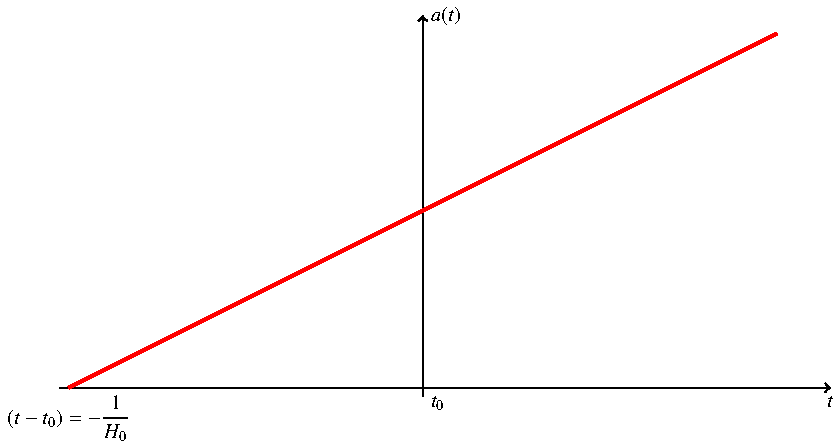
\includegraphics{chapters/tikz/friedmann-leer.pdf}
\caption{Zeitabhängigkeit des Skalenfaktors $a(t)$ in einem leeren
Universum mit $\kappa = -1$.
$a(t)$ verschwindet eine Hubble-Zeit $1/H_0$ vor heute ($t_0$).
\label{chapter:friedmann:graph:leer}}
\end{figure}
Für ein leeres Universum können wir die Friedmann-Gleichung vollständig
lösen.
Die Differentialgleichung wird dann zu
\[
\frac{\dot a(t)^2}{a(t)^2}
=
-\frac{c^2\kappa}{a(t)^2R_c^2}.
\]
Die linke Seite dieser Gleichung ist immer postiv.

\subsubsection{Leeres Universum mit positiver Krümmung: $\kappa=1$}
Für $\kappa=1$ ist die rechte Seite negativ, die Differentialgleichung
kann also gar keine Lösung haben.
Ein leeres Universum muss also automatisch $\kappa=-1$ oder $\kappa=0$
erfüllen.

\subsubsection{Leeres, flaches Universum: $\kappa=0$}
Für $\kappa=0$ ist die rechte Seite $0$, woraus man schliessen kann,
dass $\dot a(t)=0$ sein muss.
Ein leeres, flaches Universum ist also auch statisch und entspricht
damit nicht unserem Universum.

\subsubsection{Leeres Universum mit negativer Krümmung: $\kappa=-1$}
Für ein leeres Universum mit $\kappa=-1$ kann die Friedmann-Gleichung sofort
gelöst werden, man erhält
\[
\dot a(t)^2
=
\frac{c^2}{R_c^2}
\qquad\Rightarrow\qquad
\dot a(t) = \frac{c}{R_c} = 
\qquad\Rightarrow\qquad
a(t)= 1 + \frac{c}{R_c}(t-t_0).
%= 1 + H_0(t-t_0).
\]
Diese Lösung ist in Abbildung~\ref{chapter:friedmann:graph:leer} dargestellt.
Der Skalenfaktor wächst also linear mit der Zeit.
Aus den Messungen von Hubble und Humason ist die
$H_0=H(t_0)=\dot a(t_0)/a(t_0)=\dot a(t_0)$
bekannt.
Damit kann man den Skalenfaktor auch mit der Hubble-Konstanten
bestimmen:
\[
H(t) =  \frac{\dot a(t)}{a(t)} = 1 + H_0(t-t_0).
\]
Für $t=1/H_0$ wird $H(t)=0$, dann sind alle Distanzen im
Universum auf $0$ geschrumpft.


\subsection{Das nicht leere Universum}
Wenn das Universum sich ausdehnt, dehnt sich das darin enthaltene
Gas, der Staub und die Strahlung mit aus.
Ist der Energieinhalt des Universums als Funktion von $a(t)$ bekannt,
kann die Friedmann-Gleichung gelöst werden.

Neuere Messungen zeigen, dass unser Universum flach ist.
Die Rechnungen für $\kappa=1$ in den nachfolgenden Unterabschnitten
sind daher für unser Universum nicht anwendbar.
In späteren Abschnitten, insbesondere im Abschnitt über verschiedene
Komponenten des Universums, wird daher nur noch der Fall $\kappa=0$
durchgerechnet.

\subsubsection{Geschlossenes Universum}
Wir untersuchen jetzt, was für langfristige Lösungen die
Friedmann-Gleichung~\eqref{skript:friedmann:friedmann}
überhaupt erlaubt.
Insbesondere interessiert die Frage, ob ein expandierendes Universum
in eine kollabierendes Universum übergehen kann.

Zunächst beachten wir, dass die 
Friedmann-Gleichung~\eqref{skript:friedmann:friedmann}
sich nicht ändert, wenn man die Zeit umkehrt.
Dann ändert zwar $\dot a(t)$ das Vorzeichen, aber $\dot a(t)$ kommt
nur im Quadrat vor, so dass mit $a(t)$ auch $a(-t)$ die Friedmann-Gleichung
erfüllt.
Die Friedmann-Gleichung sind zeitumkehrinvariant.
Daraus folgt auch, dass ein Universum, das zum Zeitpunkt $t_1$
von Expansion zu Kontraktion übergeht, für $t>t_1$ durch
$a(t)=a(t_1-t)$ beschrieben werden kann, die Lösungsfunktion ist
also symmetrisch bezüglich $t=t_1$.
Ausserdem muss
am Punkt $t_1$ die Ableitung von $a(t)$ verschwinden, also ist
$\dot a(t_1)=0$.

Der Term $8\pi K\varrho/3c^2$ ist für ein nicht leeres Universum
immer positiv.
Der Krümmungsterm $c^2\kappa/a(t)^2R_c^2$ hat das gleiche Vorzeichen
wie $\kappa$.
Für ein negativ gekrümmtes Universum ist er immer positiv, so dass
nach der Friedmann-Gleichung ein solches Universum niemals $\dot a(t)=0$
erreichen kann, die Expansion in einem solche Universum wird also
niemals aufhören.

Die Dichte $\varrho$ der Materie ist proportional zu $a(t)^{-3}$, geht
also schneller gegen $0$ als der Krümmungsterm.
Für ein positiv gekrümmtes Universum werden also früher oder später immer
die beiden Terme auf der rechten Seite der
Friedmann-Gleichung~\eqref{skript:friedmann:friedmann}
betragsmässig gleich gross werden.
In diesem Moment folgt $\dot a(t) = 0$.
Ein expandierendes Universum mit positiver Krümmung wird also immer in eine 
Kontraktion übergehen.

Der Grenzfall ist ein Unversum mit verschwindender Krümmung oder $\kappa=0$.
In einem solchen Universum gilt
\begin{equation}
\varrho = \frac{3c^2H^2}{8\pi K}.
\label{skript:friedmann::dichte}
\end{equation}

\subsubsection{Kritische Dichte}
Der Wert der Dichte~\eqref{skript:friedmann::dichte}
für die heutige Zeit $t=t_0$ ist
\[
\varrho_c = \frac{3c^2H^2(t_0)}{8\pi K}=\frac{3c^2H_0^2}{8\pi K}
\]
und heisst die {\em kritische Dichte}.
\index{Dichte, kritische}
\index{kritische Dichte}
Ein üblicher Zahlenwert für die kritische Dichte unseres Universums ist
\[
\varrho_c = \frac{3H_0^2}{8\pi K}\simeq 10^{-26}\frac{\text{kg}}{\text{m}^3}
\]
Da ein Proton eine Masse von $1.672\cdot 10^{-27}\text{kg}$ hat, entspricht
$\varrho_c$ einer Dichte von etwa $6$ Protonen pro Kubikmeter\footnote{%
Hier nehmen wir an, dass die gesamte Materie baryonische Materie ist.
Die Existenz dunkler Materie bedeutet, dass diese Annahme falsch ist.
}.
Die kritische Dichte ist so etwas wie eine universelle kosmologische
Masseinheit für die Dichte.
Die Energiedichte
\[
\Omega=\frac{\varrho}{\varrho_c}
\]
ausgedrück in Einheiten der kritische Dichte heisst
der {\em Dichteparameter}.

\section{Komponenten}
\rhead{Komponenten}
Das reale Universum ist nicht leer, in den Beispielen haben wir den
Fall gewöhnlicher Materie bereits näher angeschaut.
Die Funktionen $\varrho(t)$ und $p(t)$ sind für verschiedene
Arten von Materie oder Energie verschieden.
Wir sprechen von verschiedenen Komponenten des Universums.
Jede Komponente hat ihre eigene Zustandsgleichung und führt
daher zu einer anderen Lösung der Friedmann-Gleichung.
In den folgenden Unterabschnitten wird jeweils die Lösung für
ein flaches Universum mit nur einer Komponente durchgerechnet.

\subsection{Materie}
Die offensichtlichste Komponente ist die sogenannte baryonische Materie.
Sie macht jedoch nur etwa 5\% des Energieinhalts des Universums aus.
Sie wird so genannt, weil ihre Masse vor allem durch die Masse der Atomkerne
bestimmt ist, aus der sie sich zusammensetzt.

Im sich ausdehnenden Universum bleibt die Masse erhalten, die Dichte wird
daher mit der dritten Potenz von $a(t)$ abnehmen, wie wir im Folgenden
nachrechnen wollen.
Ein Würfel mit Kantenlänge $l$ zur Zeit $t_0$ enthält die Masse
$m=l^3 \varrho(t_0)$.
Zur Zeit $t$ ist die Kantenlänge $a(t)l$, das Volumen $a(t)^3l^3$
und die darin enthaltene Masse $m=a(t)^3l^3\varrho(t)$.
Da die Masse erhalten bleibt, folgt
\[
l^3 \varrho(t_0)
=
a(t)^3l^3\varrho(t)
\qquad\Rightarrow\qquad
\varrho(t)=\frac{\varrho(t_0)}{a(t)^3}.
\]
Die Friedmann-Gleichung wird daher
\begin{equation}
\frac{\dot a(t)^2}{a(t)^2}
=
\frac{8\pi K\varrho_0}{3c^2a(t)^3}-\frac{c^2\kappa}{a(t)^2R_c^2}.
\end{equation}

Da die mittlere Materiedichte im Universum sehr klein ist, kann man davon
ausgehen, dass Atome praktisch nie kollidieren, dass diese Komponenten
also keinen Druck aufweist.
Staubteilchen werden trotz grösserer Masse noch seltener kollidieren.

%Die baryonische Materie wird also durch die Zustandsgleichungen
%\begin{equation}
%\varrho(t)=\frac{\varrho_0}{a(t)^3}
%\qquad\text{und}\qquad
%p(t)=0
%\end{equation}
%vollständig charakterisiert.

\subsubsection{Das flache, gasgefüllte Universum}
In einem flachen, gasgefüllten Universum ist $\kappa=0$,
der Krümmungsterm fällt weg und
es erfüllt daher die vereinfachte Friedmann-Gleichung
\[
\frac{\dot a(t)^2}{a(t)^2}
=
\frac{8\pi K\varrho_0}{3c^2 a(t)^3}.
\]
Wir lösen die Differentialgleichung, indem wir zunächst die Wurzel ziehen 
\[
\dot a(t)=\pm \sqrt{
\frac{8\pi K\varrho_0}{3c^2}
}a(t)^{-\frac{1}{2}}
\]
und dann in
\[
\sqrt{a(t)}\,
\frac{da}{dt}
=
\pm\sqrt{\frac{8\pi K\varrho_0}{3c^2}}
\]
separieren und integrieren:
\[
\int \sqrt{a}\,da
=
\int a^\frac12\,da
=
\frac23 a(t)^\frac{3}{2}
=
\pm\sqrt{\frac{8\pi K\varrho_0}{3c^2}}t + C.
\]
Auflösen nach $a(t)$ führt auf
\[
a(t)=\biggl(\pm\sqrt{\frac{6\pi K\varrho_0}{c^2}}t+C'\biggr)^{\frac23}
\]
wobei die Integrationskonstante $C'$ noch so bestimmt werden muss,
dass $a(t_0)=1$ gilt.
Dies wird erreicht mit
\begin{equation}
a(t)
=
\biggl(\pm\sqrt{\frac{6\pi K\varrho_0}{c^2}}(t-t_0) + 1\biggr)^\frac23.
\label{skript:friedmann:alter:materie}
\end{equation}

Wir möchten den Bezug zur aktuellen Ausdehnung des Universums herstellen,
dazu muss $\dot a(t_0)=H_0$ sein.
Wir berechnen daher die Ableitung
\[
\dot a(t_0)=\pm \sqrt{\frac{6\pi K\varrho_0}{c^2}}\cdot \frac23
=
\pm \sqrt{\frac{8\pi K\varrho_0}{3c^2}}
=
\pm H_0.
\]
Unser Universum expandiert, daher kommt nur das positive Vorzeichen in Frage.
Wir können den Wurzelausdruck in \eqref{skript:friedmann:alter:materie} 
ebenfalls durch $H_0$ ausdrücken.
Aus
\[
\sqrt{\frac{6\pi K\varrho_0}{c^2}}
=
\frac32
\sqrt{\frac{8\pi K\varrho_0}{3c^2}}
=
\frac32H_0
\]
folgt
\begin{equation}
a(t) = \biggl(\frac32H_0(t-t_0)+1\biggr)^\frac23
\label{skript:friedmann:alter:materie2}
\end{equation}
für den Skalenfaktor in einem materiegefüllten Universum.
Abbildung~\ref{skript:friedmann:graph:materie} zeigt den Verlauf
des Skalenfaktors.

\begin{figure}
\centering
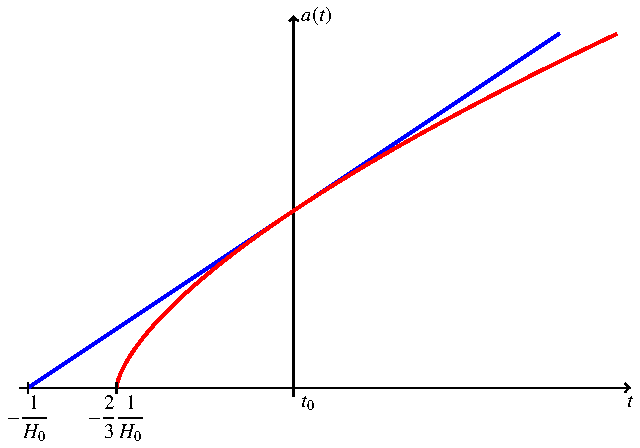
\includegraphics{chapters/tikz/friedmann-materie.pdf}
\caption{Zeitabhängigkeit des Skalenfaktors $a(t)$ ({\color{red}rot})
in einem Universum, welches nur Materie enthält.
Im Vergleich dazu {\color{blue}blau} die Entwicklung für linear von der
Zeit abhängigen Skalenfaktor, die Steigung der Geraden ist die
Hubble-Konstanten $H_0$.
Das Alter des Universums ist nur zwei Drittel der Hubble-Zeit.
\label{skript:friedmann:graph:materie}}
\end{figure}

Das Alter des Universums lässt sich damit ebenfalls ermitteln.
Dazu muss die grosse Klammer in~\eqref{skript:friedmann:alter:materie2}
verschwinden, also
\begin{equation}
\begin{aligned}
\frac32H_0(t-t_0)
&=
-1
&&\Rightarrow&
t-t_0
&=
-\frac23 \frac1{H_0}.
\end{aligned}
\label{skript:friedman:23h0}
\end{equation}
Ein materiegefülltes Universum hat daher nur ein Alter von
etwa 67\% der Hubble-Zeit. 
Setzt man die besten bekannten Werte in, erhält man 9.6Gyr,
deutlich zu wenig Zeit.

\subsection{Strahlung}
Im frühen Universum war Strahlung die dominierende Komponente.
Mit der Expansion verändert sich nicht nur die Dichte der Photonen 
analog zu einem Gas, es verändert sich auch deren Wellenlänge.
Da die Energie eines Photons proportional ist zur Wellenlänge,
nimmt die Energiedichte der Strahlung mit der vierten Potenz des
Skalenfaktors $a(t)$ ab:
\[
\varrho(t)=\frac{\varrho_0}{a(t)^4}.
\]
Die Bedeutung der Strahlung nimmt also schneller ab als jene der Materie.
% XXX Graphik, die a^-3 und a^-4 vergleicht
Dies gilt nicht nur für Strahlung, sondern auch für Teilchen, die
sich mit relativistischer Geschwindigkeit bewegen, zum Beispiel für
Neutrinos.
Daher werden solche Teilchen normalerweise ebenfalls unter dem
Strahlungsterm in der Friedmann-Gleichung subsumiert.

Die Friedmann-Gleichung für ein mit Strahlung gefülltes Universum ist
\begin{equation}
\biggl(
\frac{\dot a(t)}{a(t)}
\biggr)^2
=
\frac{8\pi K \varrho_0}{3c^2a(t)^4}
-
\frac{c^2\kappa }{a(t)^2R_c^2}.
\end{equation}
Leider lässt sich diese Differentialgleichung im allgemeinen
nicht in geschlossener Form integrieren.
Wir beschränken uns daher auf den einfacheren Spezialfall $\kappa=0$.
%wir verschieben die Diskussion der
%Lösung auf einen späteren Abschnitt, wo wir die Gleichung numerisch lösen
%können.

\subsubsection{Das flache, strahlungserfüllte Universum}
Für ein flaches Universum ist $\kappa=0$, der Krümmungsterm fällt wieder
weg und die Friedmann-Gleichung vereinfacht sich zu
\begin{equation*}
\frac{\dot a(t)^2}{a(t)^2}
=
\frac{8\pi K\varrho_0}{3c^2 a(t)^4}.
\end{equation*}
Auch hier können wir die Wurzel ziehen und mit $a(t)$ multiplizeren,
wir erhalten
\begin{equation*}
\dot a(t)
=
\sqrt{\frac{8\pi K\varrho_0}{3c^2}}\frac1{a(t)}.
\end{equation*}
Diese Gleichung lässt sich ebenfalls separieren:
\begin{align*}
a\frac{da}{dt}
&=
\sqrt{\frac{8\pi K\varrho_0}{3c^2}}
\\
\Rightarrow\qquad
\int a\,da
=
\frac12a(t)^2
&=
\sqrt{\frac{8\pi K\varrho_0}{3c^2}}t + C.
\end{align*}
Auflösen nach $a(t)$ liefert
\[
a(t)
=
\sqrt{\pm\frac{16\pi K\varrho_0}{3c^2}t + 2C}.
\]
Die Integrationskonstante muss so bestimmt werden, dass die
Anfangsbedingung $a(t_0)=1$  erfüllt ist.
Setzt man $a(t_0)=1$ ein, erhält man
\[
C
=
\mp\frac{8\pi K\varrho_0}{3c^2}t_0+1
\]
oder
\begin{equation}
a(t)
= 
\sqrt{\pm\frac{16\pi K\varrho_0}{3c^2}(t-t_0) + 1}.
\label{skript:friedmann:a(t)}
\end{equation}
Diese Wurzelfunktion beschreibt je nach gewähltem Vorzeichen ein
expandierendes oder schrumpfendes Universum.
In keinem Fall ist jedoch $\dot a(t)=0$ möglich, die Expansion kann
also nicht anhalten und in eine Kontraktion übergehen.
Da wir in einem expandierenden Universum leben, fällt der Fall
des sich zusammenziehenden Universums ausser betracht,
wir untersuchen im Folgenden nur noch das positive Vorzeichen.

\begin{figure}
\centering
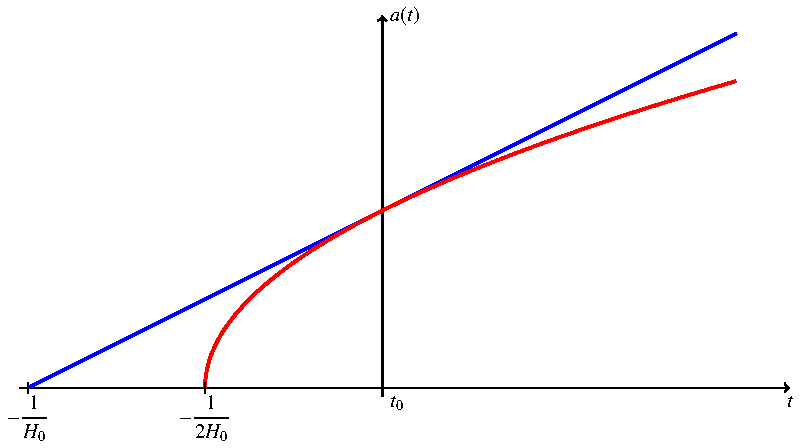
\includegraphics{chapters/tikz/friedmann-strahlung.pdf}
\caption{Zeitabhängigkeit des Skalenfaktors $a(t)$ ({\color{red}rot})
in einem Universum, welches von Strahlung dominiert ist.
Im Vergleich dazu {\color{blue}blau} die Entwicklung für linear von der
Zeit abhängigen Skalenfaktor, die Steigung der Geraden ist die
Hubble-Konstanten $H_0$.
Das Alter des Universums ist nur eine halbe Hubble-Zeit.
\label{skript:friedmann:graph:strahlung}}
\end{figure}

Wir müssen den Zusammenhang zu unserem Universum herstellen, welches
aktuell mit $\dot a(t_0)= H_0$ ausdehnt.
Dazu berechnen wir die Ableitung
\[
\dot a(t_0)=\frac{8\pi K\varrho_0}{3c^2}=H_0
\]
von~\eqref{skript:friedmann:a(t)}.
Damit können wir den Skalenfaktor auch durch die Hubble-Konstane ausdrücken,
es gilt
\begin{equation}
a(t)=\sqrt{2H_0(t-t_0)+1}.
\label{skript:friedmann:a(t):strahlung}
\end{equation}
Die Zeitabhängigkeit von $a(t)$ für ein strahlungsdominiertes Universum
ist in Abbildung~\ref{skript:friedmann:graph:strahlung} dargestellt.

Wir interessieren uns für das Alter des Universums, welches durch
die Bedingung $a(t)=0$ festgelegt wird.
Für ein expandierendes Universum kann man sofort ablesen, dass
die Expansionsgeschwindigkeit früher grösser gewesen sein muss.
Es ist also nicht zulässig, das Alter des Universums durch lineare
Extrapolation aus der aktuellen Hubble-Konstanten abzuleiten.
Vielmehr müssen wir die Zeit $t$ als Nullstelle der Funktion
\[
a(t)=\sqrt{2H_0(t-t_0)+1}
\]
bestimmt werden.
Für $t-t_0$ finden wir
\[
H_0(t-t_0)
=
-1
\qquad\Rightarrow\qquad
t-t_0 = -\frac1{2H_0}.
\]
Setzt man den besten bekannten Zahlenwert
\eqref{skript:robertson:hubble0}
für die Hubble-Konstante ein,
erhält man für das Alter des Universums
\[
t-t_0=-7.2\text{Gyr},
\]
diese Zeit ist jedoch zu kurz, unsere Sonne müsste schon etwa
2 Milliarden Jahre nach der Entstehung des Universums entstanden
sein.
Dies ist darauf zurückzuführen, dass unsere Modellierung des
Energieinhaltes unvollständig ist.



\section{Dunkle Energie}
\rhead{Dunkle Energie}
Einstein erwartete, dass das Universum statisch und unendlich alt sein
müsste Universum.
Er stellte jedoch bald fest, dass seine Gleichungen ein solches Universum
nicht beschreiben konnten.
Er fügte daher seiner Gleichung einen Term hinzu, der dies ermöglichte.
Diesen ``kosmologischen'' Term bezeichnete er nach der
Entdeckung der Expansion des Universums durch Hubble als
den grössten Fehler seines Lebens.
Heute erhält dieser Term als ``dunkle Energie'' eine neue Interpretation.

\subsection{Die kosmologische Konstante}
Als Einstein die Gleichungen der Gravitation aufstellte, war die
vorherrschende Vorstellung, dass das Universum statisch und unendlich
alt ist.
Die Friedmann-Gleichungen haben aber keine statische Lösung
für $\varrho>0$.
Einstein hat versucht, dies dadurch zu korrigieren, dass er der
linken Seite einen Summanden $\Lambda g_{\mu\nu}$ hinzufügt.
Heute wird dieser Term in den Einstein-Gleichungen auf der rechten
Seite geschrieben.

Die aus dieser modifizierten Einstein-Gleichung abgeleitete
Friedmann-Gleichung lautet jetzt
\begin{align}
\frac{\dot a(t)^2}{a(t)^2}
&=
\frac{8\pi K}{3c^2}\varrho - \frac{\kappa c^2}{a(t)^2R_c^2} + \frac{\Lambda c^2}{3},
\label{skript:friedmann:dunkleenergie}
\\
\intertext{
die Beschleunigungsgleichung wird
}
\frac{\ddot a(t)}{a(t)}
&=
-\frac{4\pi K}{3c^2}(\varrho c^2+3p) + \frac{\Lambda c^2}{3}.
\label{skript:friedmann:dunklebeschleunigung}
\end{align}
Damit $\dot a(t)=0$ ist, muss die Konstante $\Lambda$ sorgfältig auf
die Energiedichte im Universum und die Krümmung abgestimmt sein.

Aus diesem Grund war diese Korrektur der Einstein-Gleichungen nicht
wirklich erfolgreich.
Die statische Lösung von~\eqref{skript:friedmann:dunkleenergie}
ist nämlich nicht stabil.
Ein solches Universum würde bei einer winzigen Störung sofort
in eine Expansion oder Kontraktion übergehen.

Im Gegensatz zu den anderen Termen auf der rechten Seite der
Friedmann-Gleichungen nimmt der $\Lambda$-Term mit grösser werdendem
Skalenfaktor nicht ab.
Die Beschleunigungsgleichung~\eqref{skript:friedmann:dunklebeschleunigung}
zeigt, dass ein Universum mit $\Lambda > 0$ früher oder später
in eine exponentiell beschleunigte Expansion übergeht.

\subsection{Dunkle Energie}
Heute wird die Notwenigkeit des $\Lambda$-Terms von Messungen
gestützt.
Der $\Lambda$-Term als zusätzlicher Summand im Energie-Impuls-Tensor
wird {\em dunkle Energie} genannt.
Aus Messungen ist bekannt, dass er zum heutigen Zeitpunkt etwa 70\%
des Energieinhalts des Universums ausmacht.
Die dunkle Energie ist daher heute der dominante Faktor für die
Ausdehnung des Universums.
\begin{figure}
\centering
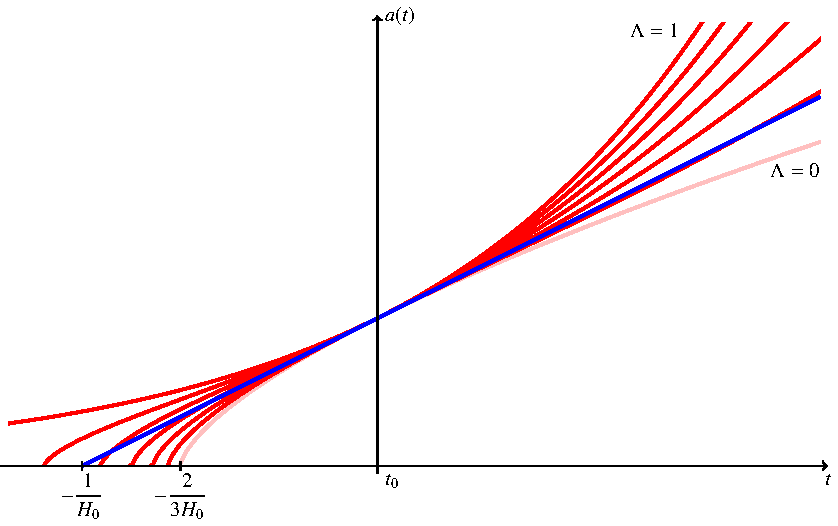
\includegraphics{chapters/tikz/darkenergy.pdf}
\caption{Zeitabhängigkeit des Skalenfaktors $a(t)$ ({\color{red}rot})
in einem Universum ohne Strahlung aber mit Materie und dunkler Energie
für verschiedene Werte von $\Lambda$.
\label{skript:friedman:graph:darkenergy}}
\end{figure}

Um zu verstehen, wie sich die dunkle Energie auf das Alter des Universums
auswirkt, berechnen wir die Entwicklung eines materiedominierten, flachen 
Universums mit verschiedenen Werten von $\Lambda$.
Die Friedmann-Gleichung dafür lautet
\[
\frac{\dot a(t)^2}{a(t)^2}
=
\frac{8\pi K \varrho_0}{3c^2a(t)^3} + \frac{\Lambda c^2}{3}
\]
Zur Zeit $t=t_0$ steht auf der linken Seite das Quadrat der Hubble-Konstanten,
es muss also gelten
\[
H_0^2
=
\frac{8\pi K \varrho_0}{3c^2} + \frac{\Lambda c^2}{3},
\]
für die Simulation müssen wir daher $\varrho_0$ und $\Lambda$ jeweils
so varieren, dass $H_0$ gleich bleibt.

Für die Berechnung ist es zweckmässig, die Hubble-Zeit als Masseinheit
für die Zeit zu verwenden, dann wird nämlich $H_0=1$.
Ausserdem wählen wir die Längeneinheit so, dass $c=1$ wird.
Ausserdem interessiert uns der genau Wert von $\varrho_0$ nicht wirklich,
entscheidend ist nur der Koeffizient von $a(t)^{-3}$ in der
Friedmann-Gleichung, die wir daher als
\newcommand{\Rho}{\mathrm{P}}
\begin{equation}
\frac{\dot a(t)^2}{a(t)^2}
=
\frac{\Rho_0}{a(t)^3} + \frac{\Lambda}{3}
\label{skript:friedmann:de:friedmann}
\end{equation}
schreiben\footnote{Das Zeichen $\Rho_0$ ist ein grosses griechisches Rho.}.
Da zur heutigen Zeit die kritische Dichte $\Rho_0$ und $\Lambda$ die gesamte
Energiedichte des Universums ausmachen, müssen sie die Bedingung
\begin{equation}
\Rho_0 + \frac{\Lambda}{3}=1
\end{equation}
erfüllen.
Damit können wir die Friedmann-Gleichung~\eqref{skript:friedmann:de:friedmann}
auch in der Form
\begin{equation}
\frac{\dot a(t)^2}{a(t)^2}
=
\biggl(1-\frac{\Lambda}3\biggr)\frac1{a(t)^3} + \frac{\Lambda}3
\label{skript:friedmann:de:simulation}
\end{equation}
schreiben.
In expliziter Form wird daraus die Differentialgleichung
\begin{equation}
\dot a(t)
=
\sqrt{
\biggl(1-\frac{\Lambda}3\biggr)\frac1{a(t)} + \frac{\Lambda}3 a(t)^2
}
\label{skript:friedmann:de:dgl}
\end{equation}
mit der Anfangsbedingung $a(t_0)=1$.

In Abbildung~\ref{skript:friedman:graph:darkenergy} sind die numerisch
gewonnenen Lösungen
der Differentialgleichung~\eqref{skript:friedmann:de:dgl} für verschiedene
Werte von $\Lambda$ dargestellt.
Man kann erkennen dass grössere Werte von $\Lambda$ zu einer stärkeren
Beschleunigung der Expansion des Universums führt.
Ausserdem wächst das Alter des Universums von $2/3H_3$ für ein
Universum ohne dunkle Energie auch über die Hubble Zeit an.
Der aktuell genaueste Wert für das Alter des Universums von 13.72Gyr
ist daher nur möglich, wenn ein beträchtlicher Teil der Energie im
Universum dunkle Energie ist.

\section{Vergleich von kosmologischen Modellen}
\rhead{Vergleich von kosmologischen Modellen}
Die Terme auf der rechten Seite der
Friedmann-Gleichung~\eqref{skript:friedmann:friedmann}
können in Einheiten der kritischen Dichte geschrieben werden.
Die verschiedenen Terme auf der rechten Seite der Friedmann-Gleichung
unterscheiden sich durch deren Veränderung in Abhängigkeit vom
Skalenfaktor $a(t)$.
Wir können die Energiedichte der einzelnen Komponenten jetzt in
Einheiten der kritischen Energie, also als ein Dichteparameter
für jede einzelne Komponenten schreiben.
Wir wählen die Bezeichungen
\begin{align*}
\Omega_{0,m}&=\text{Materie},\\
\Omega_{0,s}&=\text{Strahlung},\\
\Omega_{0,k}&=\text{Krümmung},\\
\Omega_{0,\Lambda}&=\text{dunkle Energie}.
\end{align*}
Damit können wir die Friedmann-Gleichungen schreiben als
\begin{equation}
\frac{H(t)^2}{H_0^2}
=
\Omega_{0,m}\frac1{a(t)^3}
+
\Omega_{0,s}\frac1{a(t)^4}
+
\Omega_{0,k}\frac1{a(t)^2}
+
\Omega_{0,\Lambda}.
\label{skript:friedmann:omegagleichung}
\end{equation}
Die Entwicklung eines Universums ist also vollständig durch die
vier Dichteparameter 
$\Omega_{0,m}$,
$\Omega_{0,s}$,
$\Omega_{0,k}$ und
$\Omega_{0,\Lambda}$
bestimmt.
Um verschiedene kosmologische Modelle zu vergleichen reicht es also,
die Werte der Dichteparameter zu vergleichen.

Die Summe
\[
\Omega_{\text{tot}}
=
\Omega_{0,m}
+
\Omega_{0,s}
+
\Omega_{0,k}
+
\Omega_{0,\Lambda}
\]
der Dichteparameterwerte bestimmt die Geometrie des Universums
(Tabelle~\ref{skript:friedmann:tabelle}).
\begin{table}
\centering
\begin{tabular}{|c|c|l|}
\hline
Gesamtdichte $\Omega_{\text{tot}}$&Krümmung&Universum\\
\hline
$\Omega_{\text{tot}}>1$&$\kappa = \phantom{-}1$&geschlossen\\
$\Omega_{\text{tot}}=1$&$\kappa = \phantom{-}0$&offen\\
$\Omega_{\text{tot}}<1$&$\kappa =-1$&offen\\
\hline
\end{tabular}
\caption{Zusammenhang der Materie- und Energiedichte mit der Krümmung
und der zukünftigen Entwicklung des Universums
\label{skript:friedmann:tabelle}}
\end{table}
Im Rahmen der gegenwärtig möglichen Messgenauigkeit ist
$\Omega_{\text{tot}}=1$ wir leben also höchstwahrscheinlich in
einem flachen Universum, also einem Universum mit $\Omega_{0,k}=0$.

Da unser Universum schon ziemlich alt ist, spielt die Strahlung
eine untergeordnete Rolle, $\Omega_{0,s}$ wird also vernachlässigbar
klein sein. 
Die zukünftige Entwicklung des Universums wird also bestimmt durch
das Verhältnis von $\Omega_{0,m}$ und $\Omega_{0,\Lambda}$, die
zusammen $1$ ergeben müssen.
Die Beobachtung der beschleunigten Expansion des Universums 
legt $\Omega_{0,\Lambda}\simeq 0.7$ fest.
Wegen $1=\Omega_{0,m}+\Omega_{0,\Lambda}$ folgt, dass das
Universum aktuelle Universum nur zu etwa einem Drittel aus 
Materie bestehen kann, der grössere Teil des Universums ist
dunkle Energie.

Den Materie-Anteil $\Omega_{0,m}$ beobachten wir allerdings auch
nicht.
Nur etwas 5\% der Energiedichte des Universums ist auf beobachtbare
Materie zurückzuführen.
Beobachtungen an der Bewegung von Galaxien in einem Galaxiencluster
oder der Rotationsgeschwindigkeit von Galaxien zeigen, dass zur Erzeugung
der notwendigen Gravitationskraft noch wesentlich mehr Energie vorhanden
sein muss, die wir nicht direkt beobachten können.
Was diese dunkle Materie sein könnte, die immerhin etwa einen Viertel der
Energiedichte des aktuellen Universums ausmacht, gibt es verschiedene
Hypothesen, bisher konnte keine durch experimentelle Untersuchungen
bestätigt werden.

\section{Rotverschiebung als Zeitskala%
\label{skript:section:rotverschiebung}}
\rhead{Rotverschiebung als Zeitskala}
Wir gehen heute davon aus, dass das Universum flach ist, dass die
Ausdehnung also nicht zum Stillstand kommen wird.
Insbesondere ist also $\dot a(t)>0$ für alle Zeiten $t$, die Funktion
$a(t)$ ist streng monoton wachsend.
Da $a(t)$ umkehrbar ist, kann man den Wert von $a(t)$ als kosmische
Zeitskala wählen.

Der Skalenfaktor ist der Messung jedoch nicht direkt zugänglich,
viel praktischer wäre, die Rotverschiebung als Zeitskala zu wählen.
Man definiert die Rotverschiebung $z$ durch
\[
\lambda = \lambda_0(1+z),
\]
wobei $\lambda_0$ die ursprünglich Wellenlänge und $\lambda$ die
gemessene Wellenlänge ist.
Die Expansion des Universums streckt zur Zeit $t$ ausgesandtes Licht mit
Wellenlänge $\lambda_0$ auf die Wellenlänge $\lambda=\lambda_0/a(t)$,
es folgt daher, dass
\[
1+z=\frac{1}{a(t)}
\qquad\Leftrightarrow\qquad
a(t)=\frac1{1+z}.
\]
Die Rotverschiebung $z$ kann daher ebenfalls als kosmische Zeitskala 
verwendet werden.

Natürlich ist für die Umrechnung von Rotverschiebung $z$ auf Zeit $t$
wieder eine Lösung $a(t)$ der Friedmann-Gleichung nötig.
Wenn jedoch die Zeit $t$ nicht benötigt wird, dann werden die
kosmologischen Gleichungen in der Rotverschiebungs-Zeitskala
viel einfacher.
Ersetzen wir $a(t)$ in der Gleichung~\eqref{skript:friedmann:omegagleichung},
erhalten wir
\begin{equation}
\frac{H^2}{H_0^2}
=
\Omega_{0,m}(1+z)^3
+
\Omega_{0,s}(1+z)^4
+
\Omega_{0,k}(1+z)^2
+
\Omega_{0,\Lambda}.
\label{skript:friedmann:zgl}
\end{equation}
Die Ausdehnungsgeschwindigkeit $H$ wird damit ausschliesslich eine
Funktion der Rotverschiebung.

In Abhängigkeit von der Rotverschiebung lassen sich jetzt viele Fragen
sehr einfach beantworten.
Zum Beispiel: Bei welcher Rotverschiebung geht das strahlungsdominierte
Universum in ein materiedominiertes Universum über?
Wir verwenden~\eqref{skript:friedmann:zgl} under erhalten
\[
\Omega_{0,m}(1+z)^3 = \Omega_{0,s}(1+z)^4
\qquad\Rightarrow\qquad
1+z
=
\frac{\Omega_{0,m}}{\Omega_{0,s}}.
\]
Übliche Zahlenwerte (siehe zum Beispiel Abschnitt~\ref{section:cmb:dichte})
ergeben
\begin{equation}
\frac{\Omega_{0,m}}{\Omega_{0,s}} = 9730,
\label{skript:friedmann:msequal}
\end{equation}
dies entspricht einer Zeit von $t\simeq 47\,000$ Jahren nach dem Big Bang.
Anders ausgedrückt ist heute die Materiedichte etwa $10^4$ mal grösser
als die Strahlungsdichte.



